\chapter{Evaluation}\label{ch:evaluation}

In this chapter we describe how our system is utilized to run our experiments. We provide a quantitative analysis of the data that we gathered and the comparison between the different experiment settings. Section \ref{sec:objectives} defines out experiment objectives. Section \ref{sec:methodology} describes the implementation details of how we generate our dataset and perform image classification. In section \ref{sec:results} we provide the results of our experiment. Our findings and experiment limitations are described in sections \ref{sec:findings} and \ref{sec:limitations} respectively.

\section{Objectives}\label{sec:objectives}

We hypothesize that we are able to enhance the classification accuracy of our image classifier using synthetic data for training. Multiple ratios of synthetic to real images for training are examined. Moreover, we run our experiments on multiple CNN architectures and fine-tune their hyperparameters accordingly.


\section{Methodology}\label{sec:methodology}

Our methodology is divided into 2 main parts: Dataset Generation and Image Classification. Dataset Generation is concerned with creating 3D models. Moreover, it discusses generating real and synthetic images, and how they're collected from small parts and their corresponding 3D models. Image Classification revolves around utilizing the collected images to maximize the classification accuracy of the image classifier.


\subsection{Dataset Generation}

During dataset generation, we strive to create a synthetic dataset that has a high degree of photo-realism. Simultaniously, we want to create 3D models as fast as possible to decrease the timing of the whole workflow. To achieve this balance, we aim to create an environment that is easy to model on 3D software. We attempt to eliminate light reflections and shadows and reduce the overall complexity of the scene.

\subsubsection{Creating 3D Models}
We first choose a small part that we wish for our image classifier to recognize. We use the 3D scanner to create a 3D model of the chosen small part.

We were unable to create 3D models with satisfactory quality for two reasons. Firstly, the small size of the target small parts requires a great level of precision to create an accurate 1:1 model. Secondly, the reflective surface of the small parts bounces the scanner's light off and causes the scanner to capture a lot of clutter. Figure \ref{fig:3dscans} shows a small part and its corresponding scanned 3D model. The scanner is not able to accurately scan fine details like the small part threads.

To counter this problem, we obtain readily available 3D models. We download 3D model by searching the Traceparts website\footnote{https://www.traceparts.com} for the small part's code name. Figure \ref{fig:Dataset} shows each small part and its corresponding 3D model. 

\begin{figure}[H]
\centering
  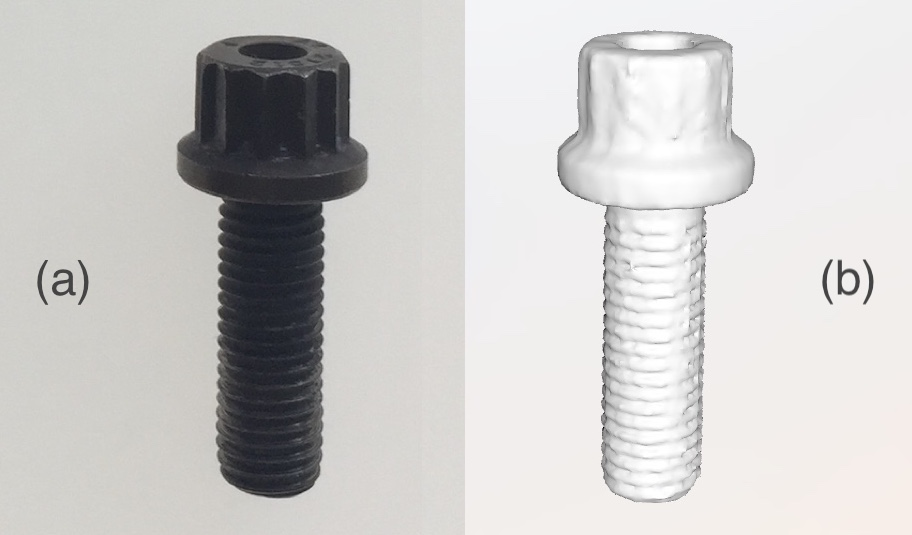
\includegraphics[width=0.75\textwidth]{3dscan}
\caption{(b) is a 3D model of the small part (a) created by 3D scanning. The 3D scanner is unable to accurately capture fine details like the small part threads as shown in (b). The 3D model is rendered without texture for clarity.}
\label{fig:3dscans}
\end{figure}

\begin{figure}[H]
\centering
  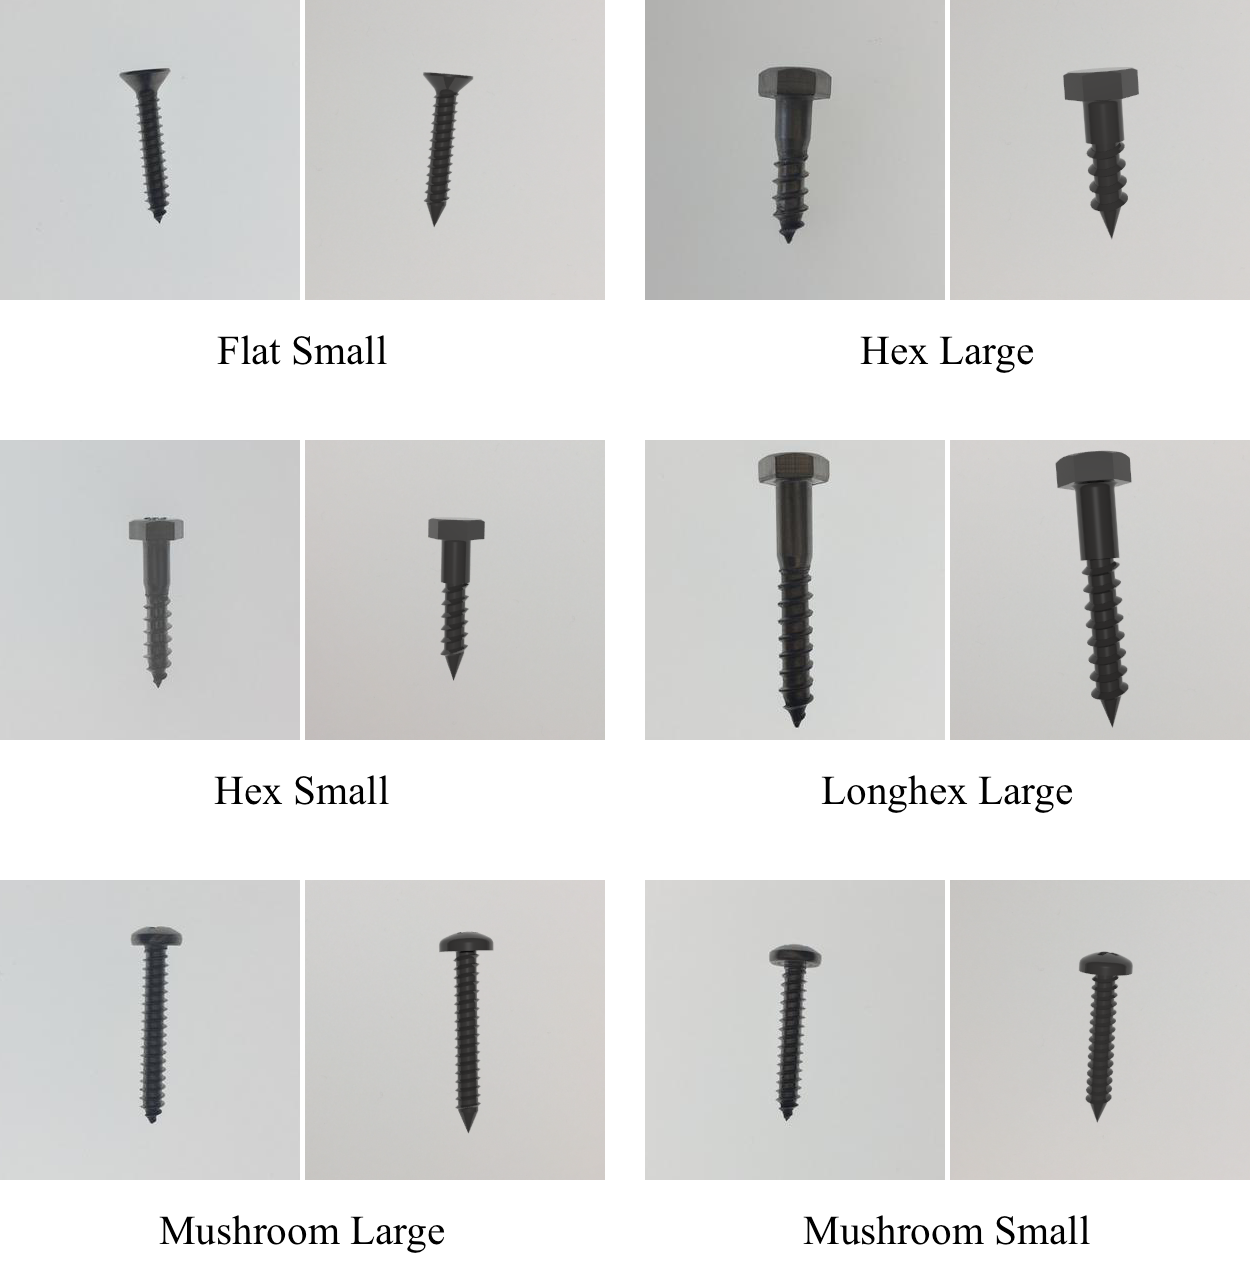
\includegraphics[width=\textwidth]{dataset}
\caption{Samples of images for each class that we use in our experiments. For each pair, the image on the left is a sample real image, while the image on the right is a sample synthetic imahe. The label under each image pair is the label we assign to the class.}
\label{fig:Dataset}
\end{figure}

\subsubsection{Generating Real Images}
We place the chosen small model on a horizontal plane and place a light source underneath. We choose a plain, white, semi-transparent plane as a background to disperse the light source coming from underneath, and distribute the light evenly accross the plane. We place the light source beneath the plane, rather than above, to eliminate any shadow that the small parts might cast. Moreover the dispersed back light provides a lighting source without casting a direct light on the objects, which might cause glare on the small part's reflective surface.

Next, we place a an iPhone over the plane, such that the small object is fully within the viewfield of the iPhone's camera. A wooden setup places the iPhone 133 mm over the plane as shown in figure [\ref{fig:RealSetup}].

Afterwards, we rotate and change the position of the small part randomly, while maintaining that the small part is fully within the viewfield of the camera. We use the iPhone's camera to take a picture of the small part. We repeat this step until we obtain the desired number of real images.

Lastly, we resize the raw real images taken by the iPhone camera to conform with the height and width required by the image classifier.

\subsubsection{Generating Synthetic Images}
We start by creating the synthetic scene in the Rhinoceros 3D modeling software. First, we take a picture of the real horizontal plane and use it as a background for our synthetic scene. We then place a synthetic lighting source underneath the plane to mimic the lighting effect of the real environment. Next, we place the 3D model on the horizontal plane of the environment.

Next, we generate a python script that uses the Rhinoceros library to manipulate 3D objects in the Rhinoceros software. The python script is the controller for the synthetic data genertor. The synthetic data generator obtains the rotation and translation ranges of the 3D model. It also specifies how many images are to be generated. For each new image, the script generates a random rotation and translation value from within the defined ranges. It then applies those transformation to the 3D model and renders a new 2D synthetic image.

\subsubsection{Dataset}
The real images generated from the small part and the synthetic images generated from the corresponding 3D model are transfered to the Training Machine where they are placed in the dataset folder.

\begin{figure}[H]
\centering
  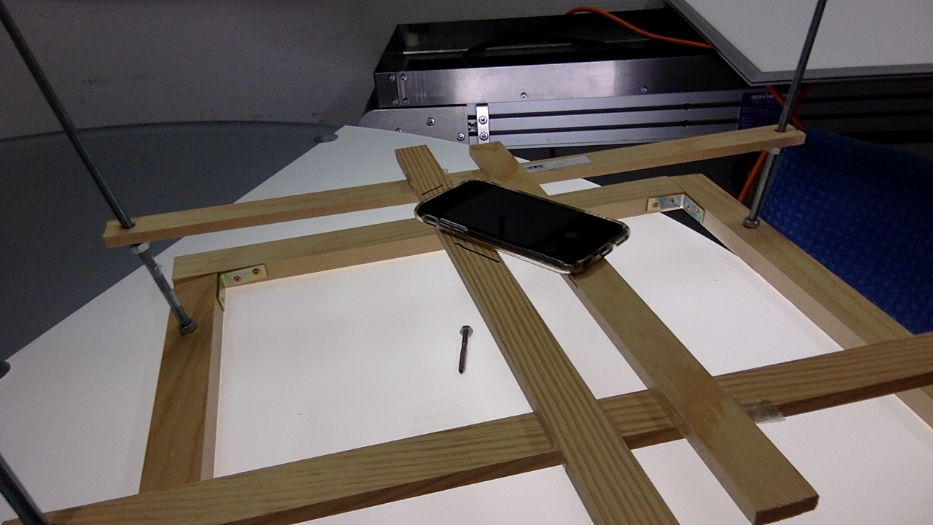
\includegraphics[width=\textwidth]{real_setup}
\caption{Set up of generating real images. An iPhone is placed on a wooden setup over a horizontal, backlit glass table with opal foils. The small part rests on the table within the viewfield of the iPhone camera.}
\label{fig:RealSetup}
\end{figure}

\begin{figure}[H]
\centering
  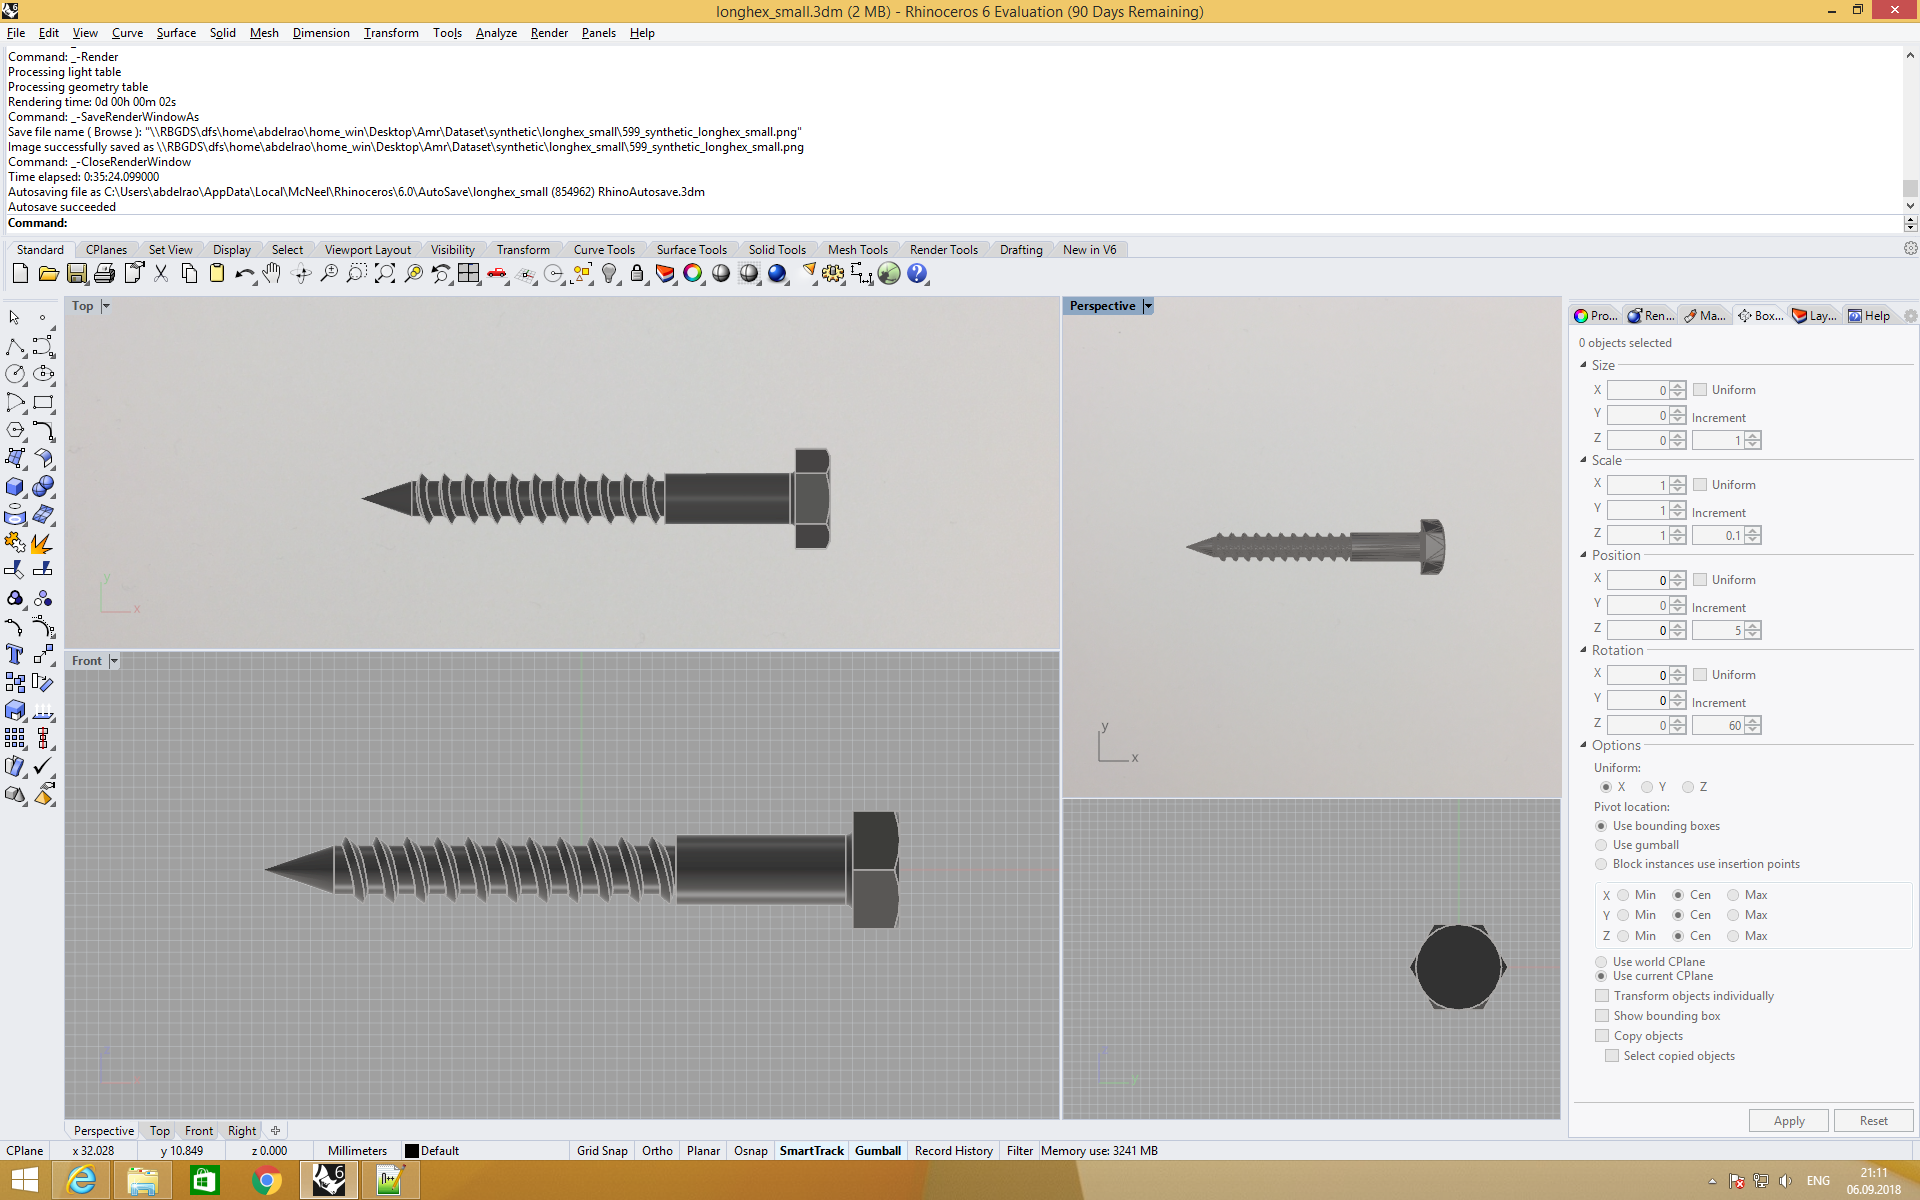
\includegraphics[width=\textwidth]{rhino_screenshot}
\caption{Synthetic scene in Rhino. The 3D model rests horizontally on a backlit plane to mimic the environment of the real setup. Sections (a) and (b) of the image depict the top view of the scene.}
\label{fig:RhinoScreenshot}
\end{figure}

\subsection{Image Classification}

The image classifier uses the images that we generate to train a convolutional neural network model to classify images of our small parts. We describe the different dataset splits that we use in our experiment. Furthermore, we present the convlutional neural models and optimizers used for image classification.

\subsubsection{Dataset Splitting}
We first split our images into a training set, a validation set and a testing set. Moreover, we determine the number of synthetic images vs the number of real images in our training set. The data split generator organizes the images in folder named after the label of their respective small part. The images are organized as shown in figure \ref{fig:FS}.

We compare the performance of 5 different ratios of synthetically enhanced training sets. Table \ref{tab:DS} describe our different dataset splits, detailing the number of images per class for each split. We generate a fully synthetic training set $\boldsymbol{R_{0}S_{100}}$, a 2.5\% real training set $\boldsymbol{R_{2.5}S_{97.5}}$, a 5\% real training set $\boldsymbol{R_{5}S_{95}}$, a 10\% real training set $\boldsymbol{R_{10}S_{90}}$, and a fully real training set $\boldsymbol{R_{100}S_{0}}$. 

\begin{table}[H]
\centering
\begin{tabular}{|l|l|l|l|l|l|}
\hline
\textbf{Dataset} & \multicolumn{1}{c|}{\textbf{\begin{tabular}[c]{@{}c@{}}Training\\ (Synthetic)\end{tabular}}} & \multicolumn{1}{c|}{\textbf{\begin{tabular}[c]{@{}c@{}}Training\\ (Real)\end{tabular}}} & \multicolumn{1}{c|}{\textbf{\begin{tabular}[c]{@{}c@{}}Training\\ (Total)\end{tabular}}} & \multicolumn{1}{c|}{\textbf{Validation}} & \multicolumn{1}{c|}{\textbf{Testing}} \\ \hline
$\boldsymbol{R_{0}S_{100}}$ & 600 & 0 & 600 & 100 & 150 \\ \hline
$\boldsymbol{R_{2.5}S_{97.5}}$ & 585 & 15 & 600 & 100 & 135 \\ \hline
$\boldsymbol{R_{5}S_{95}}$ & 570 & 30 & 600 & 100 & 120 \\ \hline
$\boldsymbol{R_{10}S_{90}}$ & 540 & 60 & 600 & 100 & 90 \\ \hline
$\boldsymbol{R_{100}S_{0}}$ & 0 & 600 & 600 & 100 & 100 \\ \hline
\end{tabular}
\caption{Different dataset splits that we use in our experiment. Each column details the number of images per class for the specified data split.}
\label{tab:DS}
\end{table}

\subsubsection{CNN Model}
For each data split, we use the VGG16 and the VGG19 \cite{simonyan2014very} convolutional neural network models. Moreover, we attempt to use the Stochastic Gradient Descent (SGD) optimizer and the Adam optimizer \cite{kingma2014adam}. We leverage the power of transfer learning \cite{pan2010survey} by using CNN models that are pre-trained on the imagenet dataset \cite{ILSVRC15}. Furthermore, we tweak our CNN models to train and evaluate images of size 500px by 500px.

\subsubsection{Hyperparameter Tuning}
For each split dataset, we fine tune the hyperparameters of the CNN model and the optimizer to maximize the classification accuracy of the output. Below is a list of hyperparameters that are optimized in the fine-tuning phase.

\begin{itemize}
  \item \textbf{Number of Frozen Layers}: Our CNN models are pre-trained on the imagenet dataset, which means that each layer is preloaded with optimized weights. During training, we freeze some of the early layers to preserve these optimized weights. We optimize our classification accuracy by fine tuning the number of frozen layers.
  \\For VGG16 we freeze 10 or 14 layers. For VGG19 we freeze 12 or 16 layers.
  \item \textbf{Batch Size}: During training, our CNN model processes the training set in batches. We fine tune our batch size between 4, 8 and 16.
  \item \textbf{Number of Epochs}: Due to the iterative nature of the training process, a CNN has to train for multiple epochs until it reaches maximum classification accuracy. We train each model for 30 epochs and observe the peak accuracy during this range.
  \item \textbf{Optimizer Learning Rate}: For stochastic gradient descent and Adam, we use a learning rate of 0.0001.
\end{itemize}


\section{Results}\label{sec:results}

Tables \ref{tab:vgg16-results} and \ref{tab:vgg19-results} provide the resulting class-wise classification accuracies of training a VGG16 network and a VGG19 network respectively. The displayed results are reached after fine-tuning the hyperparameters described in the previous section. The provided classification accuracy is the result of evaluating each CNN model using the respective testing set.


\section{Findings}\label{sec:findings}

In our experiments, we find that purely synthetic training sets generate inferior results compared to purely real training sets. A VGG16 model trained on the $\boldsymbol{R_{0}S_{100}}$ dataset has a classification accuracy of 83.556\%, a whole 16.444\% less that a VGG16 model trained on the $\boldsymbol{R_{100}S_{0}}$ dataset. However, A VGG16 trained on a training set with 10\% real data produces comparable results to a training set with purely real data. We note that while using $\boldsymbol{R_{100}S_{0}}$ dataset, the VGG16 network reached an accuracy of 100\%, while using the $\boldsymbol{R_{10}S_{90}}$ dataset resulted in an accuracy of 97.037\%. Moreover, the VGG19 network achieved an accuracy of 99.333\% using the $\boldsymbol{R_{100}S_{0}}$ dataset, compared to an accuracy of 97.222\% as a result of using the $\boldsymbol{R_{5}S_{95}}$ dataset.

Furthermore, we notice that the small parts with the highest class-wise accuracy are \textit{Flat Head} and \textit{Longhex Large}. Compared to their counterparts, those two small parts have a unique aesthetic. Hex Large and Hex small look similar, and the same goes for Mushroom Large and Mushroom Small.

\begin{table}[H]
\centering
\begin{tabular}{|l|c|c|c|c|c|c|c|}
\hline
\textbf{\begin{tabular}[c]{@{}l@{}}Dataset\end{tabular}} & \textbf{\begin{tabular}[c]{@{}c@{}}Flat\\ Head\end{tabular}} & \textbf{\begin{tabular}[c]{@{}c@{}}Hex\\ Large\end{tabular}} & \textbf{\begin{tabular}[c]{@{}c@{}}Hex\\ Small\end{tabular}} & \textbf{\begin{tabular}[c]{@{}c@{}}Long-\\ hex\\ Large\end{tabular}} & \textbf{\begin{tabular}[c]{@{}c@{}}Mush-\\ room\\ Large\end{tabular}} & \textbf{\begin{tabular}[c]{@{}c@{}}Mush-\\ room\\ Small\end{tabular}} & \textbf{Total} \\ \hline
$\boldsymbol{R_{0}S_{100}}$ & 99.333 & 48.000 & 98.667 & 96.667 & 80.667 & 78.000 & \textbf{83.556} \\ \hline
$\boldsymbol{R_{2.5}S_{97.5}}$ & 100.00 & 79.259 & 99.259 & 99.259 & 83.704 & 80.741 & \textbf{90.370} \\ \hline
$\boldsymbol{R_{5}S_{95}}$ & 100.00 & 95.833 & 100.00 & 97.500 & 90.833 & 75.833 & \textbf{93.333} \\ \hline
$\boldsymbol{R_{10}S_{90}}$ & 100.00 & 94.444 & 98.889 & 100.00 & 98.889 & 90.000 & \textbf{97.037} \\ \hline
$\boldsymbol{R_{100}S_{0}}$ & 100.00 & 100.000 & 100.00 & 100.000 & 100.000 & 100.000 & \textbf{100.000} \\ \hline
\end{tabular}
\caption{Class-wise classification accuracy of a VGG16 network trained on different ratios of synthetic data to real data.}
\label{tab:vgg16-results}
\end{table}

\begin{table}[H]
\centering
\begin{tabular}{|l|c|c|c|c|c|c|c|}
\hline
\textbf{\begin{tabular}[c]{@{}l@{}}Dataset\end{tabular}} & \textbf{\begin{tabular}[c]{@{}c@{}}Flat\\ Head\end{tabular}} & \textbf{\begin{tabular}[c]{@{}c@{}}Hex\\ Large\end{tabular}} & \textbf{\begin{tabular}[c]{@{}c@{}}Hex\\ Small\end{tabular}} & \textbf{\begin{tabular}[c]{@{}c@{}}Long-\\ hex\\ Large\end{tabular}} & \textbf{\begin{tabular}[c]{@{}c@{}}Mush-\\ room\\ Large\end{tabular}} & \textbf{\begin{tabular}[c]{@{}c@{}}Mush-\\ room\\ Small\end{tabular}} & \textbf{Total} \\ \hline
$\boldsymbol{R_{0}S_{100}}$ & 100.00 & 81.333 & 88.667 & 92.000 & 98.667 & 52.667 & \textbf{85.556} \\ \hline
$\boldsymbol{R_{2.5}S_{97.5}}$ & 100.00 & 100.00 & 86.667 & 99.259 & 99.259 & 90.370 & \textbf{95.926} \\ \hline
$\boldsymbol{R_{5}S_{95}}$ & 100.00 & 100.00 & 96.667 & 98.333 & 100.00 & 88.333 & \textbf{97.222} \\ \hline
$\boldsymbol{R_{10}S_{90}}$ & 100.00 & 90.000 & 96.667 & 98.889 & 98.889 & 96.667 & \textbf{96.852} \\ \hline
$\boldsymbol{R_{100}S_{0}}$ & 100.00 & 100.000 & 100.000 & 100.000 & 99.000 & 97.000 & \textbf{99.333} \\ \hline
\end{tabular}
\caption{Class-wise classification accuracy of a VGG19 network trained on different ratios of synthetic data to real data.}
\label{tab:vgg19-results}
\end{table}


\section{Limitations}\label{sec:limitations}

Our system is dependant on having access to the 3D model of the small parts in order to generate synthetic images. Moreover, the model's classification accuracy is dependant on the shapes of the small parts. As observed in the previous section, the class-wise accuracy for an object that is similar to other objects in the dataset is lower than an object that is aesthetically unique.